\documentclass[12pt]{article}
\usepackage[a4paper, margin=2cm]{geometry}
\usepackage{graphicx}
\graphicspath{ {../images/Sys-Log/} }
% Title information
\title{Notes de cours}
\author{Arian Dervishaj}
\date{\today}

\begin{document}
\maketitle
\pagebreak

\subsection*{Définitions}
\textbf{Big endian} : byte de poids fort au debut \\
\textbf{Little endian} : byte de poids faible au debut


\section*{Représentation des nombres entiers signés}
Utilisent une notation sur des écritures de nombres de longueur donnée.
\subsection*{Différentes façcons de resprésenter les entiers signés}
\begin{enumerate}
    \item   \textbf{Signe-magnitude} : le bit de poids fort indique le signe (0 positifs) et le restent la valeur du nombre. \\
            Pas utilisé parce qu'on ne peut pas faire de calculs avec cette méthode.
    \item   \textbf{Complément à un} : le bit de poids fort indique le signe (0 positif) et les bits restants la valeur du nombre inversé, quand la valeur est négative. \\
            Exemple : $0010 \rightarrow 2; -2 \rightarrow 1101$ \\
            Marche pas tout le temps.
    \item   \textbf{Complément à deux} : le bit de poids fort indique le signe (0 positif) et les bits restants la veleur du nombre inversé + 1, quand la valeur est négative. \\
            Exemple : Représenter -3
            \begin{enumerate}
                \item 3 = 0011
                \item Inverser : $1100$
                \item Ajouter +1 : $1101$
                \item -3 = 1101 
            \end{enumerate} 
            Exemple : Faire 2 - 3
            \begin{enumerate}
                \item $0010 + 1101 = 1111$
                \item Bit de poids fort = 1 $\rightarrow$ négatif
                \item Inverser les derniers bits : 111 $\rightarrow$ 000
                \item Ajouter +1 : 000 + 1 $\rightarrow$ 001
            \end{enumerate} 
\end{enumerate}


\section*{Algèbre de Boole}

\subsection*{Priorité des opérateurs}
\begin{enumerate}
    \item $\neg$
    \item $\land$
    \item $\lor$
    \item $\to$
    \item $\leftrightarrow$
\end{enumerate}

\begin{minipage}{0.1\textwidth}
    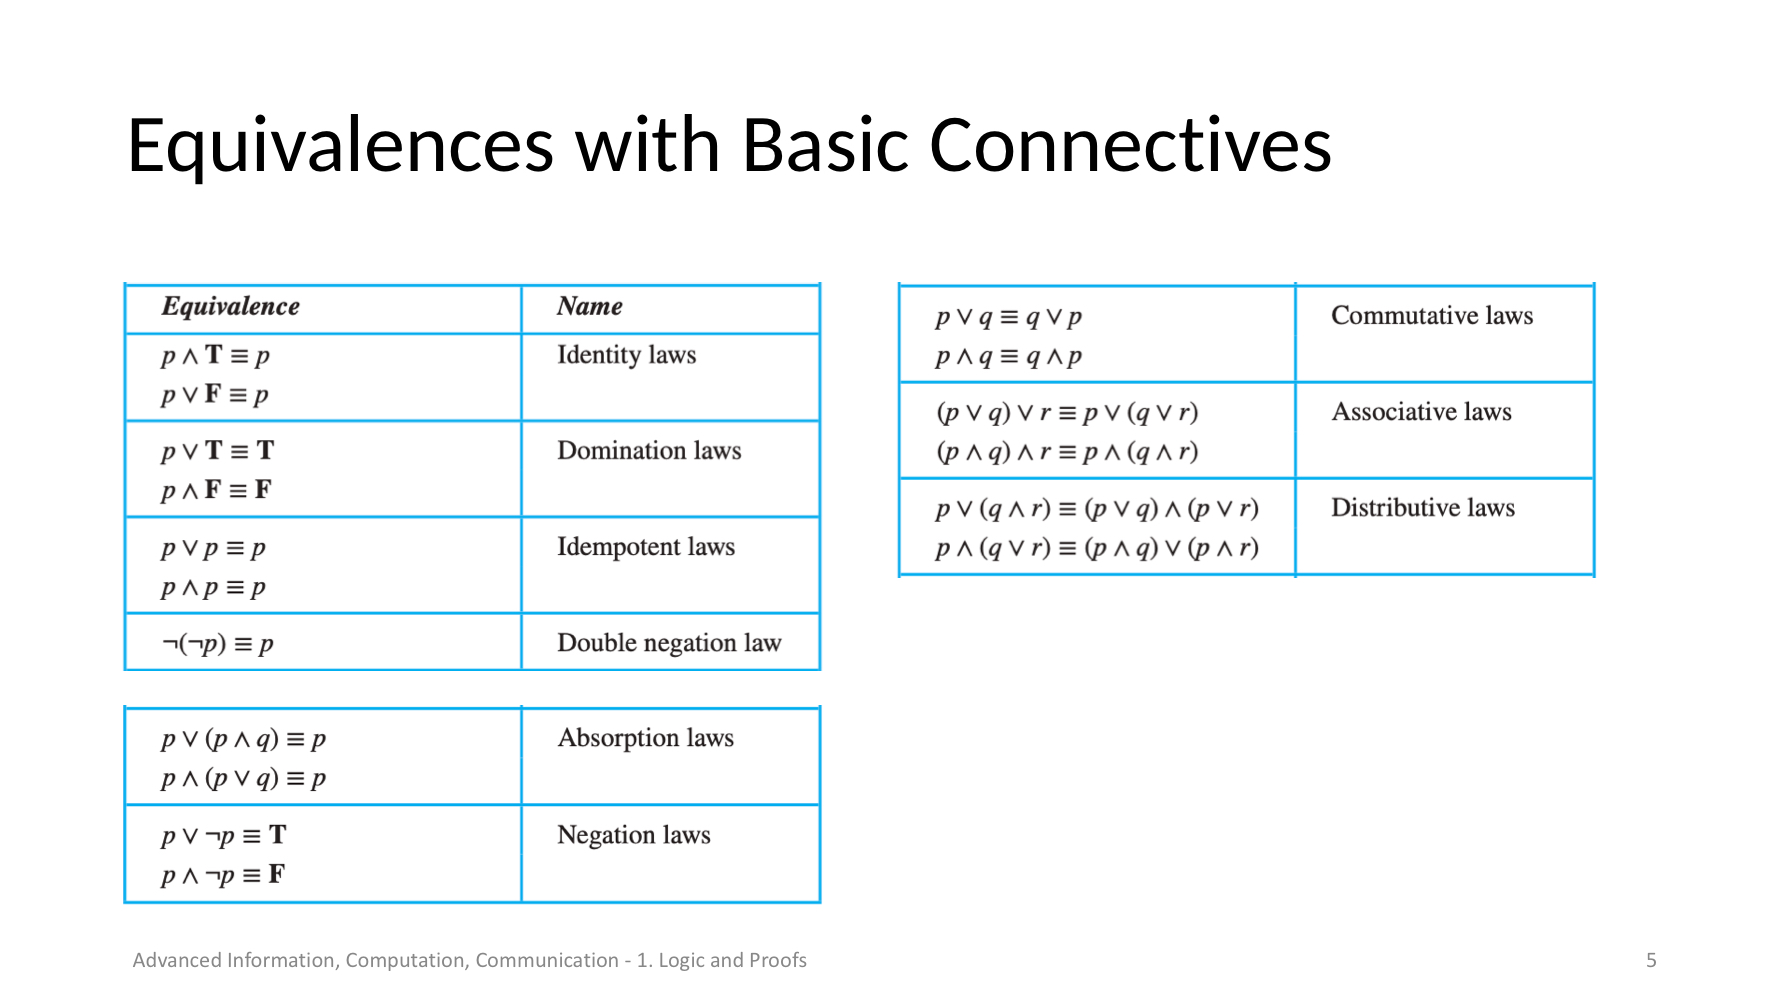
\includegraphics[scale=0.25]{Equivalence-with-basic-connective.jpeg}
\end{minipage}

\begin{minipage}{0.1\textwidth}
    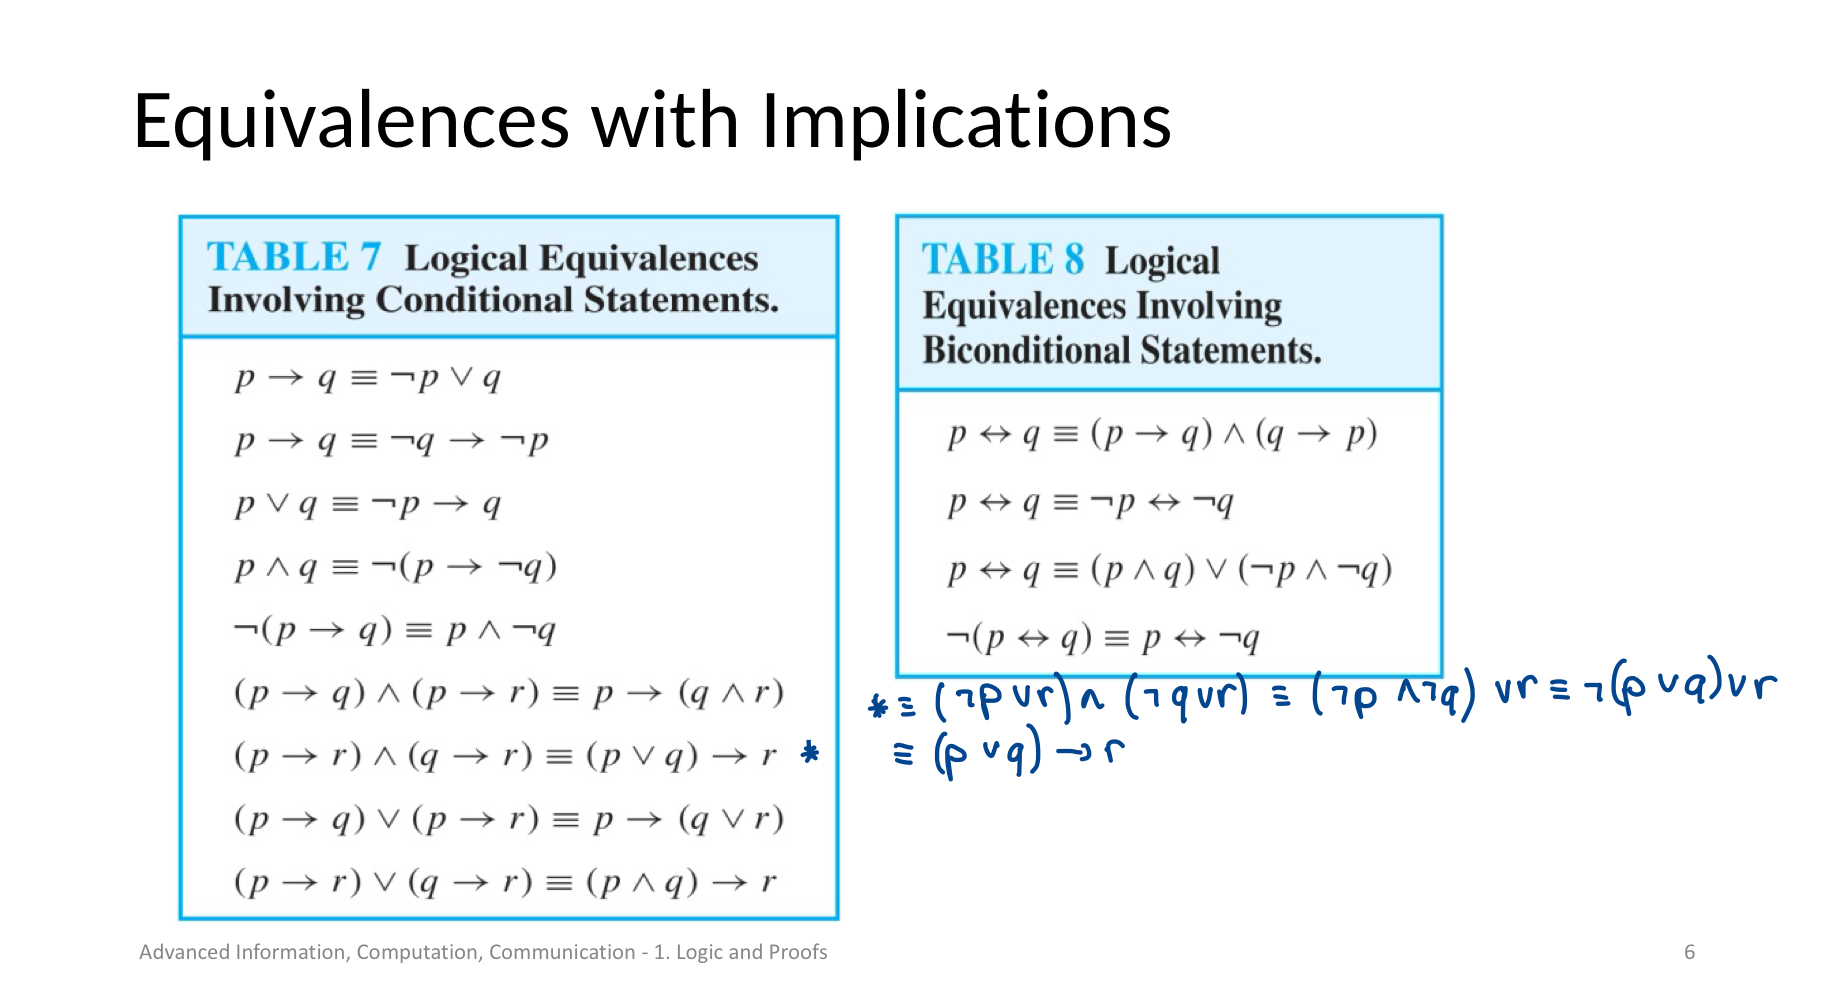
\includegraphics[scale=0.25]{Equivalence-with-implication.jpeg}
\end{minipage}
\end{document}
